\documentclass[
  captions=tableheading,
  bibliography=totoc, 
  titepage=firstiscover,
]{scrartcl}

\usepackage{blindtext} %neuer input

\usepackage{longtable} % Tabellen über mehrere Seiten

\usepackage[utf8]{inputenc} %neuer input

\usepackage{scrhack}

\usepackage[aux]{rerunfilecheck} %Warnung falls nochmal kompiliert werden muss

\usepackage{fontspec} %Fonteinstellungen

\recalctypearea{}

\usepackage[main=ngerman]{babel} %deutsche Spracheinstellung

\usepackage{ragged2e} %neuer input

\usepackage{amsmath, nccmath}

\usepackage{amssymb} %viele mathe Symbole

\usepackage{mathtools} %Erweiterungen für amsmath


\DeclarePairedDelimiter{\abs}{\lvert}{\rvert}
\DeclarePairedDelimiter{\norm}{\lVert}{\rVert}

\DeclarePairedDelimiter{\bra}{\langle}{\rvert}
\DeclarePairedDelimiter{\ket}{\lvert}{\rangle}

\DeclarePairedDelimiterX{\braket}[2]{\langle}{\rangle}{
#1 \delimsize| #2
}

\NewDocumentCommand \dif {m}
{
\mathinner{\symup{d} #1}
}


\usepackage[
  math-style=ISO,
  bold-style=ISO,
  sans-style=italic,
  nabla=upright,
  partial=upright,
  warnings-off={
    mathtools-colon,
    mathtools-overbracket,
  },
]{unicode-math}

\setmathfont{Latin Modern Math}
\setmathfont{XITS Math}[range={scr, bfscr}]
\setmathfont{XITS Math}[range={cal, bfcal}, StylisticSet=1]


\usepackage[
  locale=DE,
  separate-uncertainty=true,
  per-mode=reciprocal,
  output-decimal-marker={,},
]{siunitx}

\usepackage[autostyle]{csquotes} %richtige Anführungszeichen

\usepackage{xfrac}

\usepackage{float}

\floatplacement{figure}{htbp}

\floatplacement{table}{htbp}

\usepackage[ %floats innerhalb einer section halten
  section,   %floats innerhalb er section halten
  below,     %unterhalb der Section aber auf der selben Seite ist ok
]{placeins}

\usepackage[
  labelfont=bf,
  font=small,
  width=0.9\textwidth,
]{caption}

\usepackage{subcaption} %subfigure, subtable, subref

\usepackage{graphicx}

\usepackage{grffile}

\usepackage{booktabs}

\usepackage{microtype} %Verbesserungen am Schriftbild

\usepackage[
backend=biber,
]{biblatex}

\addbibresource{../lit.bib}

\usepackage[ %Hyperlinks im Dokument
  german,
  unicode,
  pdfusetitle,
  pdfcreator={},
  pdfproducer={},
]{hyperref}

\usepackage{bookmark}

\usepackage[shortcuts]{extdash}

%\usepackage{warpcol}


\begin{document}
    \title{ATP Übungsblatt 2}
    \author{  
    Tobias Rücker\\
    \texorpdfstring{\href{mailto:tobias.ruecker@tu-dortmund.de}{tobias.ruecker@tu-dortmund.de}
    \and}{,} 
    Paul Störbrock\\
    \texorpdfstring{\href{mailto:paul.stoerbrock@tu-dortmund.de}{paul.stoerbrock@tu-dortmund.de}}{}
    }
\maketitle
\center{\Large Abgabegruppe: \textbf{Mittw. 10-12 Uhr}}
\thispagestyle{empty}

\newpage
\tableofcontents
\thispagestyle{empty}
\newpage

\setcounter{page}{1}


\section{Aufgabe 4}

    \begin{figure}[H]
        \centering
        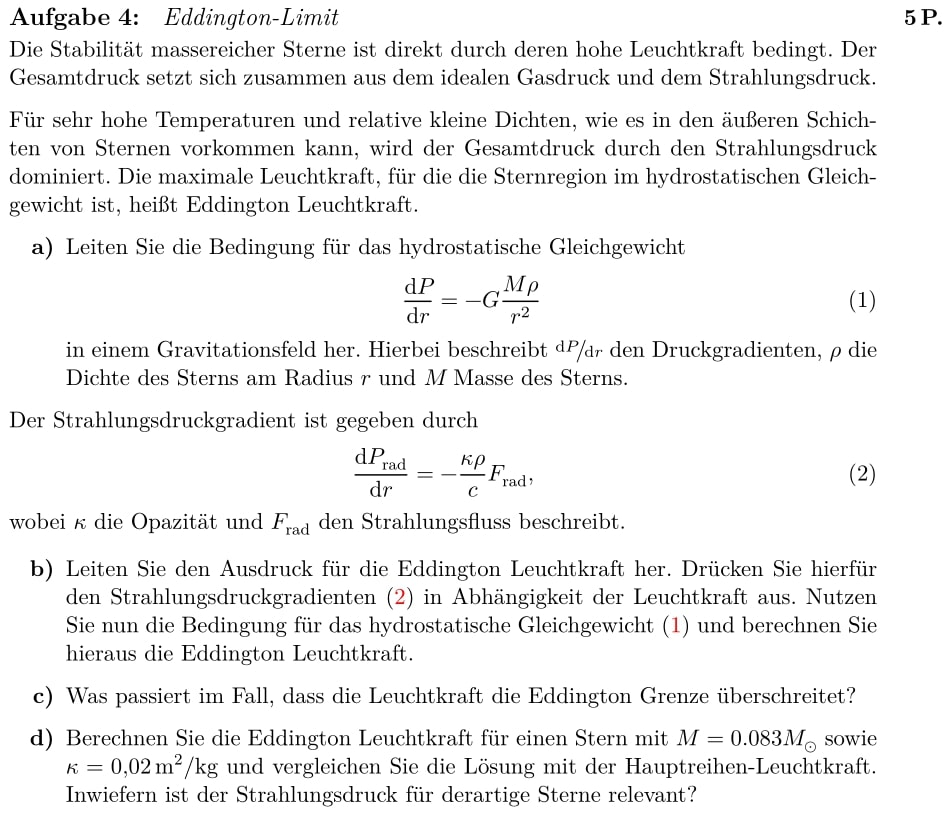
\includegraphics[width=\textwidth]{images/Aufgabe4.jpg}
        \label{fig:1}
    \end{figure}

    \flushleft{Die\;}\justifying Leuchtkraft oder Luminosität eines Sterns ist gegeben durch das Stefan-Boltzman-Gesetzt:
    \begin{align}
        L =  \sigma \cdot A \cdot T^4 \label{eq:1}
    \intertext{flushleft{Wobei\;}\justifying A die betrachtete Oberfläche, T die Oberflächentemperatur und $\sigma = \sfrac{2\pi^5 \kappa^4}{15c^2 h^3}$ die Stefan-Boltzman Konstante darstellt.
    Die Formel des Strahlungsfluss lautet
    }
        f = \frac{P_{Stern}}{A} \label{eq:2}
    \end{align}

\subsection{a)}

    \begin{align*}
        \intertext{\flushleft{Das\;}\justifying hydrostatische Gleichgewicht basiert auf das Gleichgewicht zwischen Strahlung und Druck. Demnach muss eine Variation in Druck oder Strahlung eine entsprechende
        Reaktion der anderen Kraft hervorrufen. Am Equillibrium $F_g = F_p$ muss der Druck der Strahlung gleich der Gewichtskraft sein.
        Die Gewichtskraft, die an der relevanten Schicht herrscht, ist wie folgt definiert:
        }
        dF_g &= -G \frac{M_r \mathrm{d}m}{r^2} = -G \frac{M_r \rho}{r^2}\mathrm{d}A \mathrm{d}r
        \intertext{\flushleft{Wobei\;}\justifying $G$ die Gravitationskonstante, $M_r$ die Masse der vom Radius $r$ eingeschlossenen Sphäre und $\rho$ die Dichte der Schicht an der Stelle $r$ ist.
        Der Druck ist definiert durch:
        }
        dP &= \frac{\text{Kraft(F)}}{\text{Fl\"ache(A)}} \Leftrightarrow F_p = P \cdot A
        \intertext{\flushleft{Druck\;}\justifying $p$ und Fläche sind hier jeweils variabel und vom Radius abhängig:
        }
        dF_p &= \mathrm{d}P \, \mathrm{d}A
        \intertext{\flushleft{Im\;}\justifying perfektem Gleichgewicht müssen sich beide Kräfte aufheben, demnach gilt:
        }
        dF_p - dF_g &= 0 \Leftrightarrow dF_p = dF_g\\
        \stackrel{einsetzen}{\Rightarrow} \mathrm{d}P \, \mathrm{d}A &= -G \frac{M_r \rho}{r^2}\mathrm{d}A \mathrm{d}r\\
        \Leftrightarrow \frac{\mathrm{d}P}{\mathrm{d}r} &= -G \frac{M_r \rho}{r^2}
    \end{align*}

\subsection{b)}

    \begin{align*}
        \intertext{\flushleft{Für\;}\justifying die Eddington Leuchtkraft wird der Strahlungsfluss \eqref{eq:2} benötigt, welcher in den Strahlungsdruckgradienten für $F_{rad}$ eingesetzt wird. 
        Für den Strahlungsfluss muss die Luminosität am Ort $R$ bekannt sein, welcher sich mit Formel \eqref{eq:1} bestimmen lässt.
        Werden beide Formeln in den Strahlungsdruckgradienten eingesetzt, ergibt sich für $\frac{\mathrm{d}P}{\mathrm{d}r}$:
        }
        \frac{\mathrm{d}P}{\mathrm{d}r} &= -\frac{\kappa \rho}{c} \cdot \frac{L}{A}\\
        \intertext{
            \flushleft{Wird\;}\justifying der Strahlungsdruckgradienten in Abhängigkeit von L nun nach mit der Gewichtskraft gleichgesetzt und nach L umgeformt, ergibt sich:
        }
        -\frac{\kappa \rho}{c} \frac{L}{4\pi r^2} &= -G \frac{M_r \rho}{r^2}\\
        \Leftrightarrow L &= G \frac{4\pi M_r c}{\kappa}
    \end{align*}

\subsection{c)}

    \flushleft{Eine\;}\justifying Überschreitung der Eddington Leuchtkraft liegt in der Regel einem zu hohem Strahlungsdruck zugrunde. Ein überwiegender Strahlungsdruck hat in der Regel
    eine Abstrahlung von Masse in Form von Supernovae oder planetaren Nebeln. In beiden Fällen wird mindesten eine Schicht des Stern von der sterneigenen Strahlung abgetragen. 

\subsection{d)}

    \begin{align*}
        \intertext{\flushleft{Mit\;}\justifying einer Masse von $0.083 M_{\odot}$ und einer Opazität von \SI{0.02}{\meter\squared\per\kilo\gram} ergibt sich eine Leuchtkraft von:
        } 
        L &= G \frac{4\pi 0.083M_{\odot} c}{\text{\SI{0.02}{\meter\squared\per\kilo\gram}}} = \text{\input{L.tex}}
    \end{align*}

\section{Aufgabe 5}

\begin{figure}[H]
    \centering
    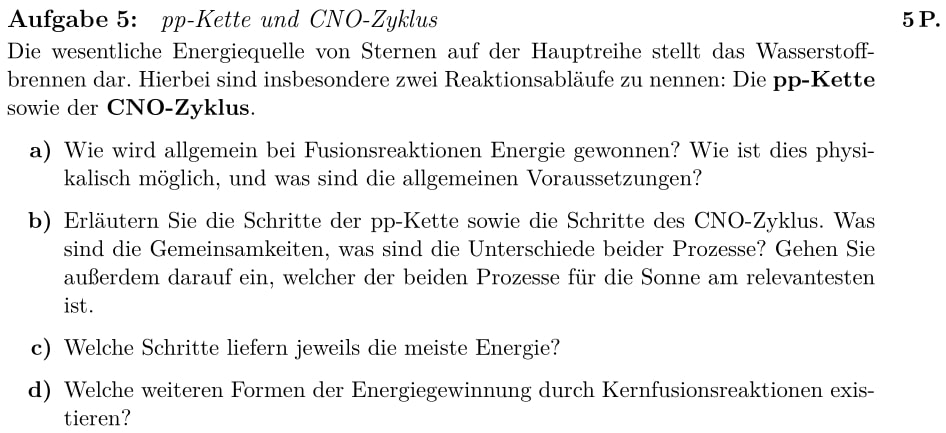
\includegraphics[width=\textwidth]{images/Aufgabe5.jpg}
    \label{fig:2}
\end{figure}

\subsection{a)}

Grundsätzlich entsteht die Energie bei einer Kernfusion daraus, dass die Bindungsenergie zweier
Reaktionspartner vor der Fusion größer als nach der Fusion ist. Dadurch wird ein Teil der Energie
in Form von Teilchen weggetragen. Das funktioniert allerdings nur bis zu einem gewissen Punkt,
da dann der Prozess der Fusion mehr Energie braucht, als sie erzeugt.

\flushleft{Die\;}\justifying Vorraussetzung für die Kernfusion sind sehr hohe Temperaturen und einen sehr hohen Druck, damit die Protonen genug Energie besitzen,
um die Coulomb-Barriere zu überwinden. Durch den quantenmechanischen Tunneleffekt sind die Protonen 
dann dazu in der Lag sich nahe genug zu kommen, um einen Fusionsprozess in Gang zu setzen. 


\subsection{b)}

pp-Kette:
Bei der pp-Kette verschmelzen zwei Wasserstoffkerne zu einem Deuteriumkern, einem Positron und einem Elektronneutrino.
Daraufhin verschmelzen ein Deuterium und ein Wasserstoff zu einem $^3$Helium und einem Gammaquant.
Der nächste Schritt, der am häufigsten Auftritt ist die Verschmelzung zweier $^3$ Helium Kerne zu
einem $^4$Helium- und 2 Wasserstoffkernen.


CNO-Zyklus:\\
Bei dem CNO-Zyklus wird in einem Kreiszyklus Stoffe in Zerfalls- und Fusionsprozessen ineinander umgewandelt.
Beginnend bei $^{12}$C mit einem Wasserstoffkern fusioniert zu $^{13}N $ und einem Gammaquant. 
Der Stickstoff zerfällt dann zu einem $^{13} C$ , einem Positron und einem Elektronneutrino.
Der Kohlenstoff funsioniert wieder mit einem Wasserstoffkern zu $^{14}N $ und einem Gammaquant.
Der Stickstoff fusioniert auch mit einem Wasserstoffkern zu einem $^{15}O $ und wieder einem Gammaquant.
Der Sauerstoff zerfällt zu einem $^{15}N $ und einem Positron sowie einem Elektronneutrino.
In dem letzte Prozess des Zyklus fusioniert der Stickstoff mit einem Wasserstoffkern zu $^{12} C $ und $^4 He$
und dann geht der Prozess mit dem Kohlenstoff wieder von vorne los.\\


\flushleft{Der\;}\justifying pp-Zyklus ist dabei der Zyklus, der bei der Sonne am stärksten vertreten ist.

\subsection{c)}
Bei der pp-Kette ist der energiereichste Übergang der Übergang von den beiden $^3$ Helium zu $^4$Helium.



\subsection{d)}


\section{Aufgabe 6}

\begin{figure}[H]
    \centering
    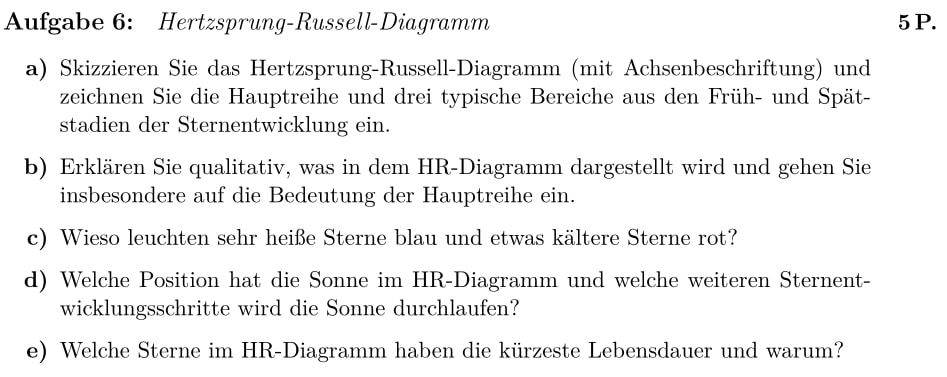
\includegraphics[width=\textwidth]{images/Aufgabe6.jpg}
    \label{fig:3}
\end{figure}

\subsection{a)}
\begin{figure}[H]
    \centering
    \caption{Hert-Russel Diagramm}
    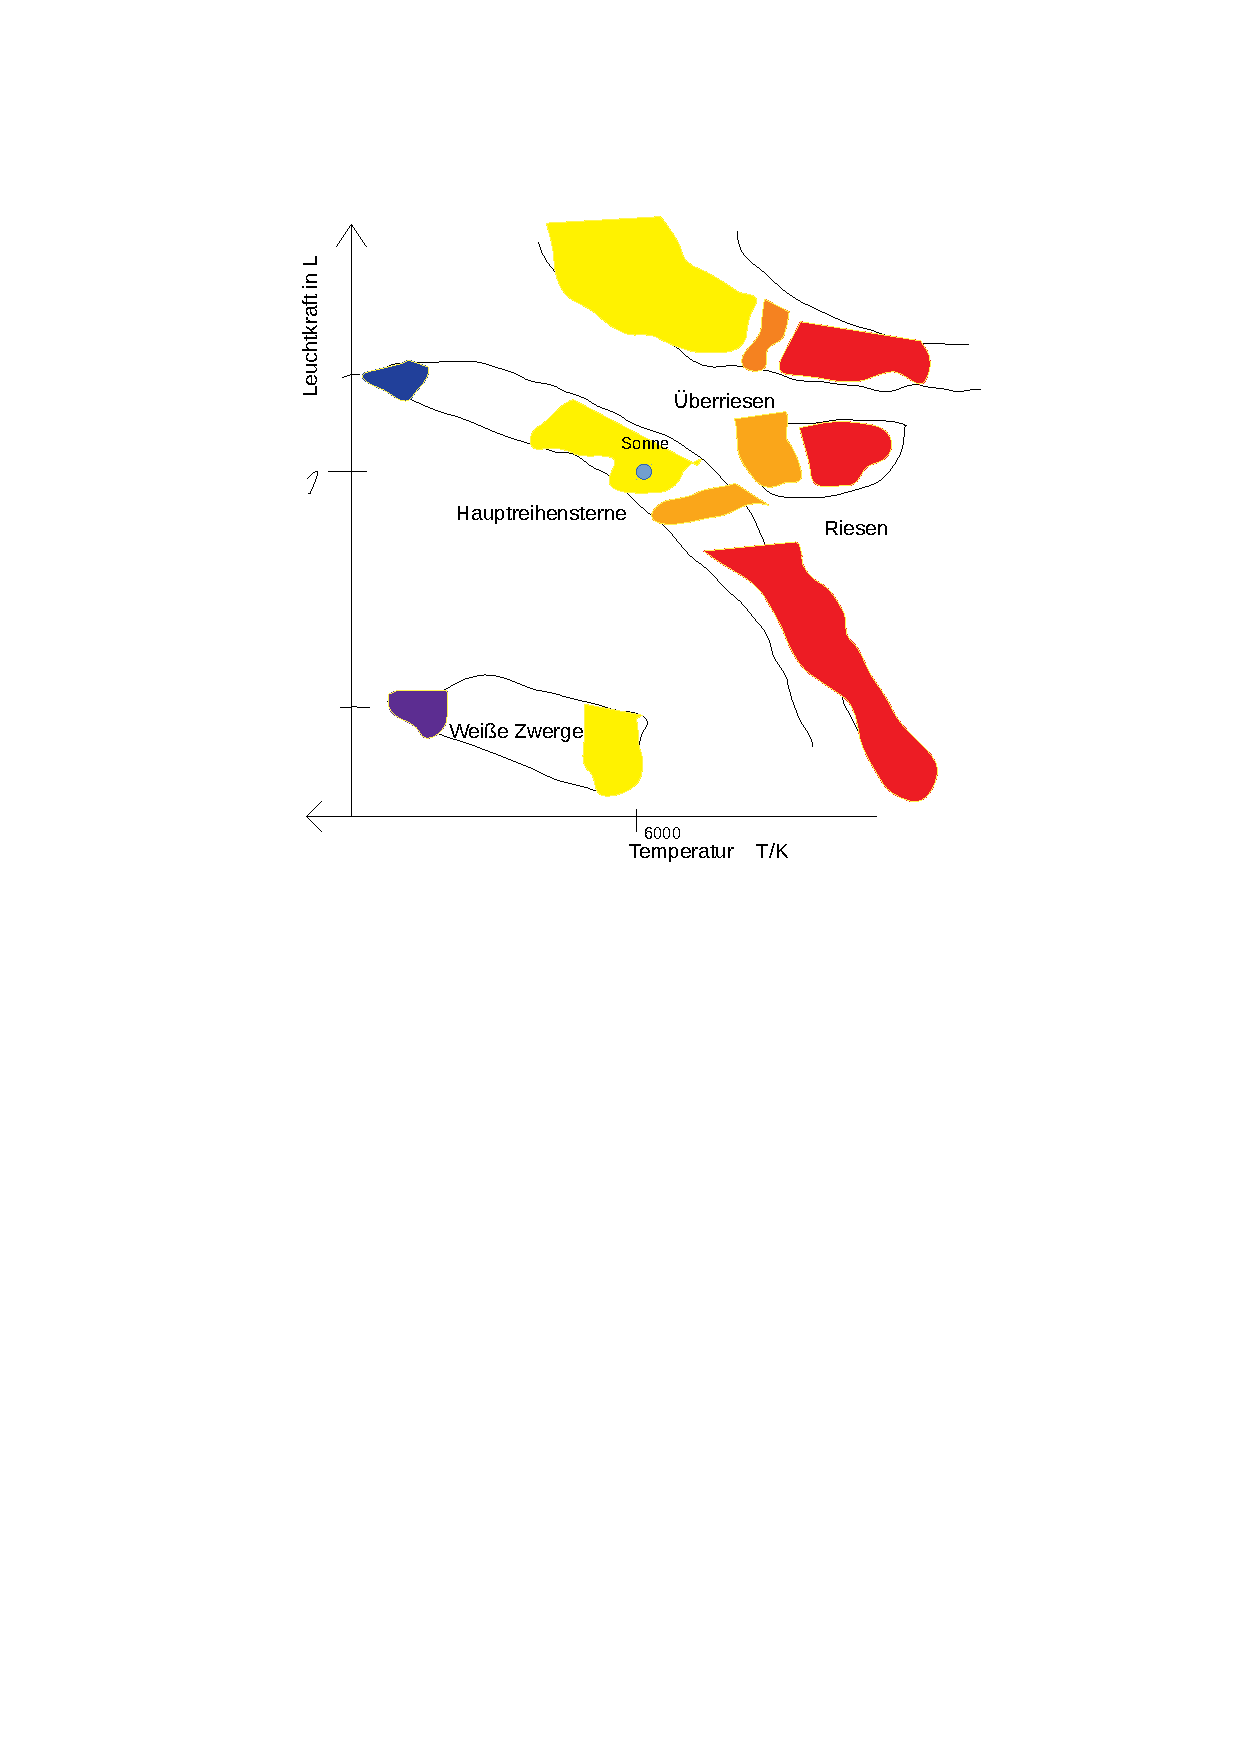
\includegraphics[width=\linewidth]{images/hertz_russel.pdf}
\end{figure}

\subsection{b)}
In dem Hertz-Russel Diagramm werden die verschiedenen Sterntypen
in Abhängigkeit ihrer Leuchtkraft und Temperatur abgebildet.
Dabei ist die Leuchtkraft logarithmisch als ein Vielfaches der
Sonnenleuchtkraft aufgetragen
Gleichzeitig werden auch die Farben der Sterne eingetragen, welche unabhängig
von ihrer Leuchtkraft sind und nur von der Temperatur hier abhängen.
Das Diagramm unterteilt sich dabei grob in 4 Bereiche.\\
Die weißen Zwerge sind die lichtschwächsten Objekte in dem Diagramm und sind Sternüberreste.\\
Riesen und Überriesen sind sehr leuchtkräftige Sterne.\\
Die Hauptreihensterne sind von großer Bedeutung, da zum einen in ihnen je nach Masse 
die pp-Kette oder der CNO Zyklus als Reaktionen stattfindet und unsere Sonne zu dieser Kategorie gehört.


\subsection{c)}

Nach dem Wienschen Verschiebungsgesetz verschiebt sich die Wellenänge der maximalen Intensität eines schwarzen Körpers
antiproportional, also $\lambda \sim 1/T $. Sterne sind näherungsweise schwarze Körper und damit
verschiebt sich bei höheren Temperaturen die Wellenlänge in den blauen Spektralbereich und bei 
niedrigeren in den Roten.

\subsection{d)}

Die Sonne gehört im HR-Diagramm zu den Hauptreihensternen. Im Laufe ihrer Zeit wird die Sonne 
zu einem roten Riesen, sobald ihr Wasserstoff für den pp-Prozess ausgeht.
Danach wird sie zu einem weißen Zwerg. Sobal der weiße Zwerg seine gesamte Restenergie abgestrahlt hat
wird dieser zu einem schwarzen Stern.

\subsection{e)}

Die Sterne mit der kürzesten Lebensdauer sind die Überriesen. Ihr Brennprozess im Kern ist aufgrund ihrer
immensen Gravitation wesentlich Intensiver. Dadurch wird der Wasserstoff in ihnen wesentlich schneller verbraucht.




\end{document}